\documentclass[11pt]{article}
\usepackage[margin=1in]{geometry}
\usepackage[T1]{fontenc}
\usepackage{lmodern}
\usepackage{amsmath,amssymb}
\usepackage{microtype}
\usepackage{booktabs}
\usepackage{graphicx}
\usepackage{xcolor}
\usepackage{tikz}
\usepackage{pgfplots}
\pgfplotsset{compat=1.17}
\usetikzlibrary{arrows.meta,positioning,shapes.geometric,fit,backgrounds}
\usepackage[numbers,sort&compress]{natbib}
\usepackage[colorlinks=true,linkcolor=blue!50!black,citecolor=blue!50!black,urlcolor=blue!50!black]{hyperref}

\newcommand{\repo}{\url{https://github.com/abdelkabirouadoukou/si-loop}}
\newcommand{\repoline}{\href{https://github.com/abdelkabirouadoukou/si-loop}{\raisebox{-0.2ex}{
\includegraphics[height=1.6ex]{docs/img/github-icon.pdf}}~\texttt{si-loop}}}

\title{Persistent Online False-Discovery Control for a Guarded\\[2pt] Self-Improvement Loop: A Process-Restart Bug, Its Fix,\\[2pt] and a Pilot Case Study}
\author{Abdelkabir Ouadoukou\thanks{Independent researcher. Contact: abdelkabir.ouadoukou@gmail.com.
Substantial AI assistance was used; see the disclosure at the end.}}
\date{November 2026\\[9pt]{\small\repoline}}

\begin{document}
\sloppy
\maketitle
\vspace{-1.2em}

\begin{abstract}
Study~3 \citep{ouadoukou2026study3} ran a live language-model proposer behind SI-Loop's sealed judge, with an online false-discovery monitor (e-LOND, \citealp{xu2024elond}) attached in \emph{monitor} mode: it logged alarms but never blocked an accept. Study~4 asks the next question on that kernel's own roadmap: can the loop also improve the code that proposes and judges its own changes (arm~A1), under the same monitor now running in \emph{enforced} mode. Building the arm-A1 runner surfaced three bugs, none in the kernel itself. The one this paper is about: \texttt{kernel/orchestrator.py} constructs a fresh online false-discovery budget, $\mathrm{ELond}(t{=}0,d{=}0)$, every time a new \texttt{Orchestrator} object is built, which happens every time the command-line runner is launched as a new process. Within one continuous run the budget tightens correctly; across the separate process launches a long-lived pilot is actually made of, it silently resets, handing back a generous early-test allowance each time and undermining the anytime-valid guarantee the monitor exists to provide. We fix this with \texttt{study4/fdr\_replay.py}: a function that replays every past correctness-path test already recorded in the run's own JSON ledger, using the hit/no-hit outcome the monitor itself recorded, and injects the reconstructed state through \texttt{TwoStageJudge}'s existing optional constructor parameter, with no edit to \texttt{kernel/}. We verify the fix two ways: a unit test that builds two independent \texttt{Orchestrator} instances sharing one ledger and checks the second continues the first's budget exactly; and a live run, where we computed the next cycle's required significance level from the ledger \emph{before} running it ($0.0012158542\ldots$) and the live run matched it exactly. A 13-cycle live pilot against \texttt{openai/gpt-oss-120b} (arm~A1) then shows both the bug and the fix side by side in the same ledger: one process boundary where the level incorrectly repeats, and a later one where it correctly continues. The pilot accepted nothing. Seven candidates reached the correctness path and were blocked by the enforced monitor, including one with $p_{\text{better}}=0.9999$, because zero prior discoveries had earned the sequence any room; the required level fell from $0.0304$ to $0.00062$ over those seven tests. We report this as the intended, anytime-valid behaviour of a cold-started budget, not a malfunction, and we make no claim about recursive self-improvement capability: this is an infrastructure correctness result and a transparent, mid-session pilot, in the spirit of Study~3's own disclosed judge defects.
\end{abstract}

\section{Introduction}
\label{sec:intro}

A guarded self-improvement loop that runs for a long time, or across many separate invocations, tests many candidate patches sequentially. Each test is a statistical decision: does this patch's measured pass-rate gain reflect a real improvement, or noise. If the number of tests is fixed in advance, classical multiple-comparisons correction applies. An open-ended loop has no such fixed number: the stream of tests is generated adaptively, by a proposer whose next move depends on the outcome of the last one, and it can run indefinitely. This is exactly the setting \emph{online} false-discovery control is built for \citep{xu2024elond,ramdas2023gtsavi}: control the long-run false-discovery rate over an unbounded, adaptively generated sequence of tests, validly at every stopping time, not just at a horizon fixed beforehand.

Studies~2 and~3 \citep{ouadoukou2026study2,ouadoukou2026study3} built this monitor into SI-Loop's two-stage judge but ran it in \emph{monitor} mode: every correctness-path test is still scored and logged, but a failing e-value never blocks the accept. The monitor was observational, not a gate. Study~4 asks whether the loop can go further and improve the code that proposes and judges its own changes (arm~A1, editing a small policy file under \texttt{agent/meta/}), and its own design decisions include switching this specific monitor to \emph{enforced} mode: closing exactly the gap Study~3 left open.

\paragraph{The problem this paper reports.} Enforcing a monitor is only as good as the state it enforces against. We found, while wiring the arm-A1 runner, that the kernel's online false-discovery budget is not a property of the \emph{study}; it is a property of the \emph{process}. \texttt{Orchestrator.\_\_init\_\_} (\texttt{kernel/orchestrator.py}) always constructs \texttt{self.elond = ELond(cfg.fdr\_alpha)}, a fresh object with its two counters, $t$ (tests so far) and $d$ (discoveries so far), both zero. Nothing anywhere persists or restores them. A long pilot is not one process; it is several, launched minutes or hours apart as rate limits, pauses, and ordinary command-line use dictate. Each launch silently re-granted the generous initial allowance an online-FDR schedule reserves for a sequence's first few tests, exactly the thing the monitor is supposed to prevent happening more than once.

\paragraph{Contributions.}
\begin{itemize}\setlength\itemsep{1pt}
\item A precise statement and live demonstration of the process-restart gap in \texttt{kernel/stats.py}'s \texttt{ELond}, a pre-existing property of the kernel shared by Studies~2 and~3, not introduced by this work (Section~\ref{sec:evolution}).
\item A fix, \texttt{study4/fdr\_replay.py}, that reconstructs the exact $(t,d)$ state from the ledger's own history and injects it through an existing, unused extension point in \texttt{kernel/pipeline.py}'s \texttt{TwoStageJudge}, with no edit to \texttt{kernel/} (Section~\ref{sec:fix}).
\item Two independent verifications of the fix: a controlled unit test, and a live run whose first required significance level was predicted from the ledger before the run and matched exactly (Section~\ref{sec:fix}).
\item A 13-cycle live pilot (arm~A1, \texttt{openai/gpt-oss-120b}) that captures the bug and the fix in the same ledger, and documents what an enforced, cold-started online-FDR budget does to a real, adaptively generated test sequence: nothing was accepted, and the required bar tightened by roughly a factor of fifty over seven tests (Section~\ref{sec:case}).
\end{itemize}

This is an infrastructure-correctness paper with one honest case study attached, not a result about language-model self-improvement. No patch was accepted in the pilot, the pilot's own code changed mid-session as these bugs were found, and we do not pool it with any pre-registered claim; that is the same stance Study~3 took toward its own pilot run and toward the two judge defects (D1, D2) it found and disclosed.

\section{Design evolution: Studies 1 through 3}
\label{sec:evolution}

\paragraph{Study 1 \citep{ouadoukou2026study1}.} A toy closed loop (hypernetwork, curriculum, guarded judge, competitive workspace) on synthetic few-shot regression. Its main lesson for this line of work was methodological: an over-cautious judge that rejects most rounds can look simply unhelpful in aggregate statistics, and a rising curve on its own does not establish that improving the \emph{improver} was what helped. Study~1 has no online false-discovery control; its gate is a single fixed-sample test per round.

\paragraph{Study 2 \citep{ouadoukou2026study2}.} Introduced the kernel this work still runs on: zero-trust git worktrees, a seven-layer patch defence, a two-stage paired non-inferiority gate (an anytime-valid screen on batch~A, then a strict confirm on an independent batch~B), a frozen cycle-0 anchor with a margin budget, a held-out problem family, a three-tier sealed verifier with honeypots, and a hash-chained ledger with circuit breakers. \texttt{kernel/stats.py}'s \texttt{ELond} (e-LOND online false-discovery control \citep{xu2024elond}, valid under the arbitrary dependence an adaptive loop produces) was built in at this stage, wired into \texttt{kernel/pipeline.py}'s confirm stage, but exercised only on a synthetic world with a scripted proposer. \texttt{cfg.fdr\_mode} already had three values, \texttt{off}, \texttt{monitor}, and \texttt{enforce}; Study~2's own ablation runs used \texttt{monitor}.

\paragraph{Study 3 \citep{ouadoukou2026study3}.} Replaced the scripted proposer with a live model (\texttt{openai/gpt-oss-120b} via Groq) on arm~A0 (solver patches only), in six pre-registered replicates. Every replicate produced at least one correctness-path accept; transfer to the held-out family was rare (one of six met the pre-declared criterion). Two judge defects were found and disclosed: D1, a utility-path clause that was always true because the verifier reports zero tokens for every candidate; and D2, a verifier suite that missed a tie-break bug in one task family. Relevant here: \texttt{fdr\_mode} stayed at \texttt{monitor} throughout Study~3. Its own discussion names this directly: \emph{``The monitor that could have flagged overfitting ran in monitor mode, and we have not extracted its flags for every run. It should be enforced \ldots before any stronger result is made.''} Study~4's design draft (\texttt{study4/DESIGN\_DRAFT.md}) accordingly declares enforcement a precondition, not an option, before any improver-arm run: this paper is the first time \texttt{fdr\_mode="enforce"} has been exercised against a live, adaptively generated proposal stream on this kernel.

\section{The process-restart gap and its fix}
\label{sec:fix}

\subsection{How the online budget works}

\texttt{ELond} (\texttt{kernel/stats.py}) implements e-LOND \citep{xu2024elond}. Test $t$ is declared a discovery iff its e-value clears
\[
\alpha_t = \alpha \cdot \gamma_t \cdot (D_{t-1}+1), \qquad \gamma_t = \frac{6}{\pi^2 t^2} \ \text{(the default, anytime-valid schedule, with } \textstyle\sum_t \gamma_t \le 1\text{)},
\]
where $D_{t-1}$ is the number of discoveries strictly before test $t$. Two counters are enough to reproduce the whole trajectory: $t$, the number of tests run, and $d=D_t$, the number of discoveries so far. \texttt{level()} returns the level the \emph{next} test will be run at, from the current $(t,d)$; \texttt{test(log\_e)} increments $t$, compares the supplied e-value against that level, and increments $d$ on a hit. \texttt{kernel/pipeline.py}'s \texttt{TwoStageJudge} calls \texttt{self.elond.test(log\_e\_up(b,c))} once for every candidate that reaches the correctness path on its confirm batch, and (when \texttt{fdr\_mode="enforce"}) rejects outright on a miss, regardless of what the ordinary paired gate decided.

\subsection{The gap}

\texttt{Orchestrator.\_\_init\_\_} always runs \texttt{self.elond = ELond(cfg.fdr\_alpha)}. No code path anywhere calls \texttt{ELond}'s own \texttt{state()}/\texttt{load()} methods, which exist and are unused. A fresh \texttt{Orchestrator}, built every time \texttt{run\_study4.py~--run} is launched as a new process, therefore always starts at $(t,d)=(0,0)$, regardless of how many correctness-path tests the same output directory's ledger already records. This is a property of \texttt{kernel/orchestrator.py} and \texttt{kernel/pipeline.py} as they stood for Studies~2 and~3 as well; it was simply never exercised in \texttt{enforce} mode before, and monitor mode's own correctness does not depend on the budget being right (it never gates on it).

\subsection{The fix}

\texttt{study4/fdr\_replay.py} provides two functions.

\begin{itemize}\setlength\itemsep{1pt}
\item \texttt{replay\_elond\_state(ledger\_path, fdr\_alpha)} returns a fresh \texttt{ELond(fdr\_alpha)} advanced through every past \texttt{"end"} ledger record that carries a \texttt{detail.fdr} entry, in file order. For each such record it applies \emph{exactly} \texttt{ELond.test}'s own update rule, \texttt{t += 1; d += int(hit)}, using the \texttt{hit} boolean the monitor itself already recorded, not a recomputed e-value. The result is, by construction, identical to the state a single continuously running process would have reached after the same sequence of tests.
\item \texttt{attach\_persistent\_fdr\_budget(orch, ledger\_path)} calls the above and assigns the result to \emph{both} \texttt{orch.elond} and \texttt{orch.judge.elond}. These are the same object at construction time (\texttt{TwoStageJudge} is built with \texttt{self.elond} as an argument), but replacing only one of the two attributes after the fact would leave the orchestrator and the judge looking at two different budgets: a mistake worth naming because it is easy to make and silent if made.
\end{itemize}

No file under \texttt{kernel/} is edited. \texttt{TwoStageJudge.\_\_init\_\_} (\texttt{kernel/pipeline.py}) already accepts an optional, pre-built \texttt{elond} parameter; this is a deliberate extension point, not a workaround. \texttt{study4/run\_live.py} calls \texttt{attach\_persistent\_fdr\_budget} immediately after constructing the \texttt{Orchestrator}, before any cycle runs, for both arms A0 and A1.

\begin{figure}[t]
\centering
\resizebox{\linewidth}{!}{%
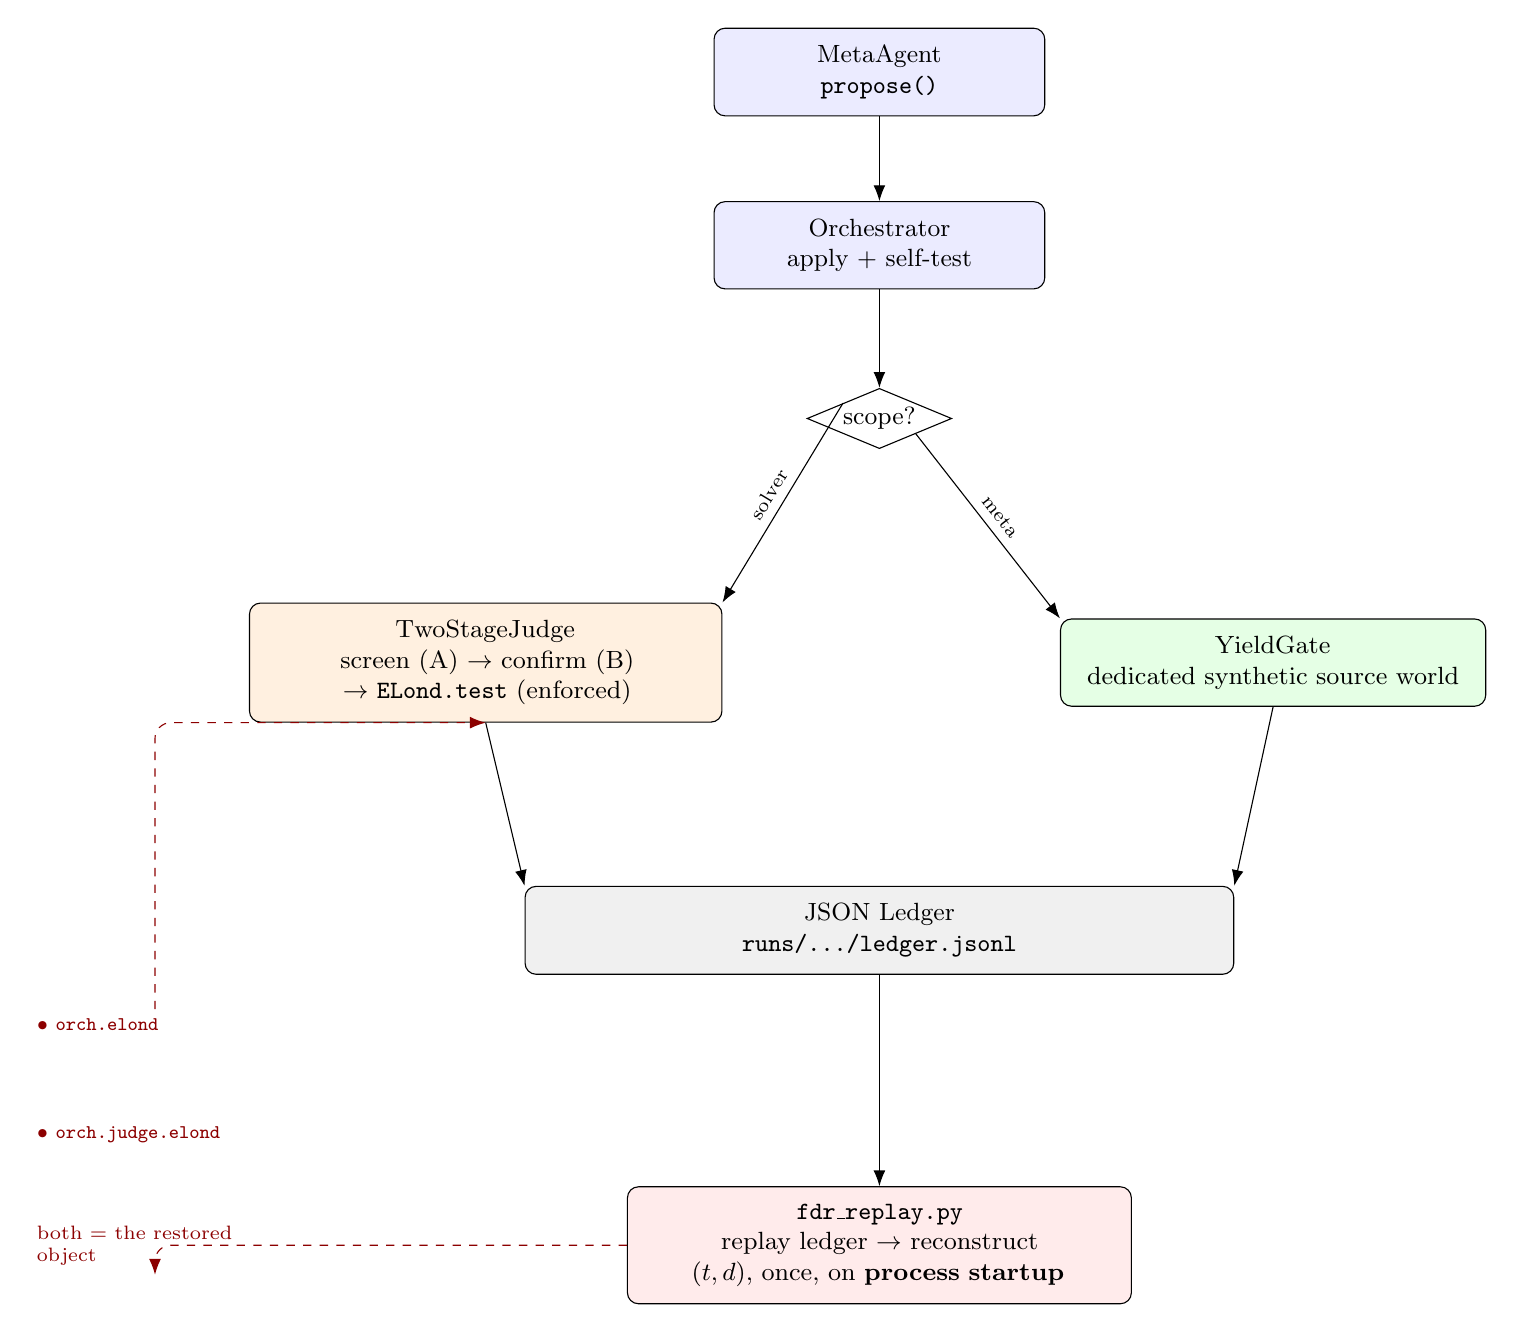
\begin{tikzpicture}[
  box/.style={draw, rounded corners, align=center, font=\small, inner sep=2.2mm},
  decision/.style={draw, diamond, aspect=2.4, align=center, font=\small, inner sep=1pt},
  annot/.style={align=left, font=\scriptsize, text width=30mm, color=red!55!black},
  >={Latex[length=2mm]},
  ]
  % main chain, absolute coordinates in cm, generous vertical gaps throughout
  \node[box, fill=blue!8, minimum width=4.2cm] (meta) at (0,11.5) {MetaAgent\\\texttt{propose()}};
  \node[box, fill=blue!8, minimum width=4.2cm] (orch) at (0,9.3) {Orchestrator\\apply + self-test};
  \node[decision] (scope) at (0,7.1) {scope?};

  \node[box, fill=orange!12, minimum width=6.0cm, text width=5.4cm] (judge) at (-5,4)
       {TwoStageJudge\\screen (A) $\to$ confirm (B)\\$\to$ \texttt{ELond.test} (enforced)};
  \node[box, fill=green!10, minimum width=5.4cm, text width=4.8cm] (yield) at (5,4)
       {YieldGate\\dedicated synthetic source world};

  \node[box, fill=gray!12, minimum width=9.0cm] (ledger) at (0,0.6)
       {JSON Ledger\\\texttt{runs/\ldots/ledger.jsonl}};

  \node[box, fill=red!8, minimum width=6.4cm, text width=5.8cm] (replay) at (0,-3.4)
       {\texttt{fdr\_replay.py}\\replay ledger $\to$ reconstruct $(t,d)$, once, on \textbf{process startup}};

  % the two assignments this fix makes, placed in open space well clear of every box
  \node[annot] (lbl1) at (-9.2,-0.6) {$\bullet$ \texttt{orch.elond}};
  \node[annot] (lbl2) at (-9.2,-2.0) {$\bullet$ \texttt{orch.judge.elond}};
  \node[annot] (lbl3) at (-9.2,-3.4) {both $=$ the restored object};

  % main (solid) flow
  \draw[->] (meta) -- (orch);
  \draw[->] (orch) -- (scope);
  \draw[->] (scope.north west) -- node[above, sloped, font=\scriptsize] {solver} (judge.north east);
  \draw[->] (scope.south east) -- node[above, sloped, font=\scriptsize] {meta} (yield.north west);
  \draw[->] (judge.south) -- (ledger.north west);
  \draw[->] (yield.south) -- (ledger.north east);
  \draw[->] (ledger.south) -- (replay.north);

  % feedback (dashed), routed through the open left margin, clear of every box above
  \draw[->, dashed, red!55!black, rounded corners=2mm] (replay.west) -| (lbl3.south);
  \draw[->, dashed, red!55!black, rounded corners=2mm] (lbl1.north) |- (judge.south);
\end{tikzpicture}}
\caption{One cycle. A solver-scope patch goes through the two-stage judge and, on the correctness path, the enforced e-LOND test (folded into the same box: it is one call inside \texttt{TwoStageJudge.judge}, not a separate pipeline stage); a meta-scope patch (arm A1, \texttt{agent/meta/policy.py}) is instead judged by \texttt{YieldGate} against a dedicated synthetic world, never the live repository (a second bug fixed this session, \texttt{study4/yield\_gate.py}). Every outcome is written to the ledger regardless of branch. The dashed path, executed once per process at startup, not per cycle, is this paper's fix: \texttt{fdr\_replay.py} replays the ledger's history into a reconstructed $(t,d)$ and installs it on both \texttt{orch.elond} and \texttt{orch.judge.elond}, the same object at construction time, before the next cycle can call \texttt{ELond.test}.}
\label{fig:arch}
\end{figure}

\begin{figure}[t]
\centering
\resizebox{0.98\linewidth}{!}{%
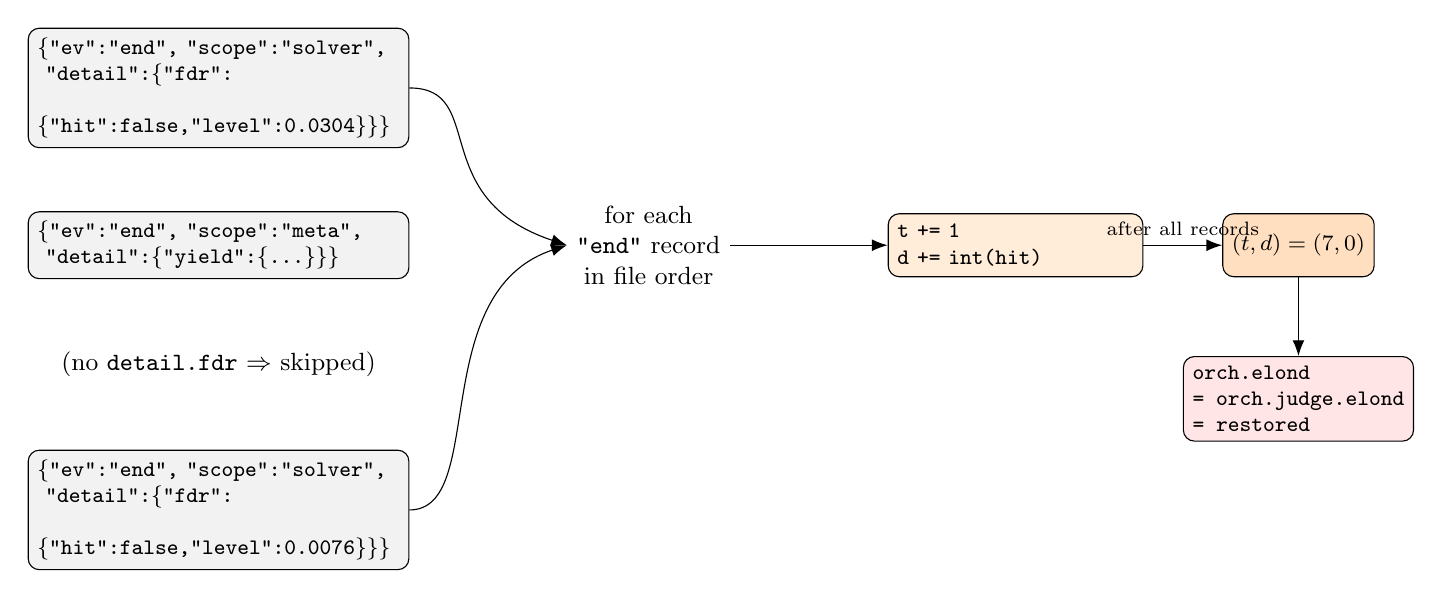
\begin{tikzpicture}[
  node distance=8mm and 10mm,
  box/.style={draw, rounded corners, align=left, font=\footnotesize\ttfamily, minimum height=8mm},
  lbl/.style={font=\small, align=center},
  ]
  \node[box, fill=gray!10, text width=46mm] (rec1) {\{"ev":"end", "scope":"solver",\\ \ "detail":\{"fdr":\\ \ \ \{"hit":false,"level":0.0304\}\}\}};
  \node[box, below=of rec1, fill=gray!10, text width=46mm] (rec2) {\{"ev":"end", "scope":"meta",\\ \ "detail":\{"yield":\{\ldots\}\}\}};
  \node[lbl, below=of rec2] (skip) {(no \texttt{detail.fdr} $\Rightarrow$ skipped)};
  \node[box, below=of skip, fill=gray!10, text width=46mm] (rec3) {\{"ev":"end", "scope":"solver",\\ \ "detail":\{"fdr":\\ \ \ \{"hit":false,"level":0.0076\}\}\}};
  \node[lbl, right=20mm of rec2] (loop) {for each\\\texttt{"end"} record\\in file order};
  \node[box, right=20mm of loop, fill=orange!15, text width=30mm] (acc) {\texttt{t += 1}\\\texttt{d += int(hit)}};
  \node[box, right=of acc, fill=orange!25] (state) {$(t,d) = (7,0)$};
  \node[box, below=10mm of state, fill=red!10] (inject) {\texttt{orch.elond}\\\texttt{= orch.judge.elond}\\\texttt{= restored}};

  \draw[-{Latex[length=2mm]}] (rec1.east) .. controls +(10mm,0) and +(-18mm,6mm) .. (loop.west);
  \draw[-{Latex[length=2mm]}] (rec3.east) .. controls +(10mm,0) and +(-18mm,-6mm) .. (loop.west);
  \draw[-{Latex[length=2mm]}] (loop) -- (acc);
  \draw[-{Latex[length=2mm]}] (acc) -- node[above, font=\scriptsize] {after all records} (state);
  \draw[-{Latex[length=2mm]}] (state) -- (inject);
\end{tikzpicture}}
\caption{\texttt{replay\_elond\_state}: every ledger \texttt{"end"} record that carries a \texttt{detail.fdr} entry (a correctness-path test actually ran) contributes one $(t{+}{=}1, d{+}{=}\mathrm{int(hit)})$ step, in file order; records with no such entry (a meta-scope yield test, or a cycle that never reached the confirm stage) are skipped. The reconstructed state is installed on \emph{both} \texttt{orch.elond} and \texttt{orch.judge.elond}, which are the same object at construction time, so a partial update would silently desynchronise them.}
\label{fig:replay}
\end{figure}

\section{Pilot case study}
\label{sec:case}

A pilot was run against the live model (\texttt{openai/gpt-oss-120b} via Groq), arm~A1, over four separate process launches in one session, output directory \texttt{runs/study4\_live}. \textbf{This is a debugging-phase pilot, not a pre-registered replicate.} The code itself changed partway through: a local self-test environment issue was fixed by setting up the project's virtual environment, \texttt{study4/yield\_gate.py}'s dedicated-synthetic-source fix was applied, and this paper's own fix was built and wired, all \emph{during} this session, the same way Study~3's pilot exposed D1. It is reported in full, kept unpooled, the same stance \texttt{results/study3/}\allowbreak\texttt{DEVIATIONS.md} takes toward that pilot.

\subsection{Overall outcome}

Thirteen cycles ran; none was accepted (Table~\ref{tab:breakdown}). Every judged cycle proposed a change to \texttt{agent/lib.py} (scope \texttt{solver}); arm~A1's live model never attempted an edit to \texttt{agent/meta/policy.py} in this pilot, despite its system prompt stating that path is allowed. With only 13 cycles this is not evidence either way, only something to watch in a longer run.

\begin{table}[h]
\centering\small
\caption{All 13 cycles of the pilot, by rejection cause.}
\label{tab:breakdown}
\begin{tabular}{@{}lrp{0.68\linewidth}@{}}
\toprule
Reject reason & Count & Cause \\
\midrule
\texttt{selftest} & 2 & pre-fix environment bug (sandboxed self-test could not see a user-site \texttt{pytest}); not a judge outcome \\
\texttt{fdr} & 7 & enforced online false-discovery control (this paper's subject) \\
\texttt{no\_gain} & 2 & ordinary two-stage-judge rejection, no measured pass-rate improvement \\
\texttt{unconfirmed} & 2 & screened well on batch A, did not hold up on independent batch B \\
\bottomrule
\end{tabular}
\end{table}

\subsection{The bug and the fix, side by side, in one ledger}

Seven candidates reached the correctness path and were tested by \texttt{ELond}. Table~\ref{tab:fdr} lists all seven in ledger order, with the process boundary each one followed. Tests~1 and~2 are separated by a process restart under the \emph{pre-fix} code: test~2 incorrectly repeats test~1's level exactly, $0.030396\ldots$, instead of the lower level a continuing sequence would use: the empirical signature of the bug. Tests~2, 3, and~4 run inside one process (the restart gap being measured is specifically \emph{across} launches, not within one), and correctly tighten relative to each other. Tests~4 and~5 are separated by a second process restart, this time under the \emph{fixed} code: test~5's level was computed from the ledger \emph{before} that run (predicted $0.0012158542\ldots$ from $t{=}4,d{=}0$), and the live run matched it exactly.

\begin{table}[h]
\centering\small
\caption{Every correctness-path test in the pilot, in ledger order. $p_\text{better}$ and $\delta$ are the ordinary paired gate's own statistics on that candidate's confirm batch ($n=48$); neither cleared $\alpha_t$ (column `level'), so every row is a miss (`hit' = false) under the enforced monitor, regardless of how convincing the ordinary gate found it.}
\label{tab:fdr}
\begin{tabular}{@{}rrrlll@{}}
\toprule
Test & $p_\text{better}$ & $\delta$ & Level $\alpha_t$ & Boundary crossed before this test & Correct? \\
\midrule
1 & 0.9688 & $+0.083$ & $0.030396$ & (first test of the pilot) & -- \\
2 & 0.9688 & $+0.083$ & $0.030396$ & \textbf{process restart, pre-fix} & \textbf{no (repeats test 1)} \\
3 & 0.9922 & $+0.125$ & $0.007599$ & (same process as test 2) & yes \\
4 & 0.9961 & $+0.146$ & $0.003377$ & (same process as test 3) & yes \\
5 & 0.9688 & $+0.083$ & $0.001216$ & \textbf{process restart, post-fix} & \textbf{yes (predicted in advance)} \\
6 & 0.9922 & $+0.125$ & $0.000844$ & (same process as test 5) & yes \\
7 & 0.9999 & $+0.250$ & $0.000620$ & (same process as test 6) & yes \\
\bottomrule
\end{tabular}
\end{table}

Figure~\ref{fig:levels} plots the required level against test index on a log scale. Final state: $(t,d)=(7,0)$; the next correctness-path test in this ledger needs $\alpha_8 \approx 0.000475$, an e-value above roughly $2100$, to be declared a discovery.

\begin{figure}[t]
\centering
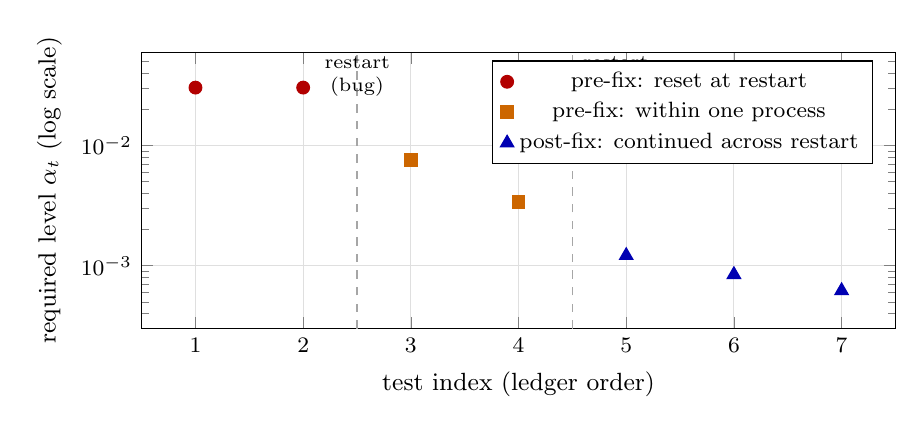
\begin{tikzpicture}
\begin{semilogyaxis}[
  width=0.92\linewidth, height=0.42\linewidth,
  xlabel={test index (ledger order)}, ylabel={required level $\alpha_t$ (log scale)},
  xmin=0.5, xmax=7.5, xtick={1,2,3,4,5,6,7},
  ymin=0.0003, ymax=0.06,
  grid=major, grid style={gray!25},
  legend pos=north east, legend style={font=\footnotesize},
  tick label style={font=\footnotesize}, label style={font=\small},
  ]
  \addplot[only marks, mark=*, mark size=2.3pt, color=red!70!black]
    coordinates {(1,0.030396355092701333) (2,0.030396355092701333)};
  \addlegendentry{pre-fix: reset at restart}
  \addplot[only marks, mark=square*, mark size=2.3pt, color=orange!80!black]
    coordinates {(3,0.007599088773175333) (4,0.003377372788077926)};
  \addlegendentry{pre-fix: within one process}
  \addplot[only marks, mark=triangle*, mark size=2.8pt, color=blue!70!black]
    coordinates {(5,0.0012158542037080532) (6,0.0008443431970194815) (7,0.0006203337774020681)};
  \addlegendentry{post-fix: continued across restart}
  \draw[dashed, gray!70] (axis cs:2.5,0.0003) -- (axis cs:2.5,0.06);
  \node[font=\scriptsize, align=center, text width=24mm] at (axis cs:2.5,0.045) {process\\restart\\(bug)};
  \draw[dashed, gray!70] (axis cs:4.5,0.0003) -- (axis cs:4.5,0.06);
  \node[font=\scriptsize, align=center, text width=24mm] at (axis cs:4.9,0.045) {process\\restart\\(fixed)};
\end{semilogyaxis}
\end{tikzpicture}
\caption{Required significance level $\alpha_t$ for each correctness-path test, in ledger order. The flat segment at tests 1--2 is the bug: a process restart handed back the generous first-test level instead of continuing the decline. From test~4 to test~5, a second process restart correctly continues the same declining sequence, because \texttt{fdr\_replay.py} had been applied by then; test~5's level was computed from the ledger and published before that run, and matched.}
\label{fig:levels}
\end{figure}

\subsection{A concrete rejected candidate}

Test~4's candidate, inspected directly in \texttt{runs/study4\_live/runs/proposal\_history.jsonl}, implemented two functions the seed deliberately leaves as \texttt{raise NotImplementedError} placeholders, \texttt{two\_sum} and \texttt{flatten}, both correctly and without hard-coding, matching their docstrings exactly. Its confirm-batch statistics, $b=4,c=0,n=48$, $p_\text{better}=0.9961$, would clear the ordinary gate's own correctness-path threshold ($p_\text{improve\_min}=0.95$) comfortably. The enforced monitor rejected it anyway, because the cumulative budget at that point required $\alpha_4=0.003377$ and the candidate's e-value did not reach it. The mechanism blocking this candidate was the statistics, not a flaw in the candidate.

\section{Discussion and future work}
\label{sec:discussion}

\paragraph{What this shows.} An enforced, cold-started e-LOND budget does exactly what it is specified to do: it does not treat a single convincing-looking test, however convincing, as a confirmed discovery when the sequence has not yet earned the room for one. Table~\ref{tab:fdr}'s test~7 ($p_\text{better}=0.9999$) is the clearest illustration available in this pilot. This directly closes the gap Study~3 named in its own limitations: a monitor that only logs cannot have this effect, because it never gates.

\paragraph{What it does not show.} Thirteen cycles, zero discoveries, is not evidence that arm~A1 cannot produce an accepted patch, nor that the enforced setting is miscalibrated. With $\gamma_t \propto 1/t^2$ and $d=0$ throughout, the budget available to test $t$ shrinks whether or not the candidates being tested are improving, and Table~\ref{tab:fdr} shows they were getting \emph{more} convincing ($\delta$ rising from $0.083$ to $0.250$) while the bar rose faster still. This is the known cost of anytime-valid control under a cold start: safety is bought with power, and the only thing that replenishes the budget, a factor of $(d+1)$ on every subsequent $\alpha_t$, is an actual discovery. A sequence that never gets one stays conservative by design.

\paragraph{A trap to name and avoid.} The natural-looking response to a starved budget, lowering $p_\text{improve\_min}$ or $\alpha$ until something clears the bar, is exactly the kind of post-hoc, result-driven parameter change the pre-registration discipline in this repository exists to prevent (Studies~2 and~3 record their own post-hoc deviations explicitly rather than making them silently). Any recalibration belongs in a new pre-registration, decided before seeing further results, not as a reaction to this pilot's zero.

\paragraph{Mitigations worth evaluating, not yet adopted.} \texttt{ELond} already supports a \texttt{uniform} schedule ($\gamma_t = 1/\text{horizon}$) as an alternative to the default \texttt{inv\_sq}; a declared horizon trades the indefinite-runtime guarantee for a flatter, less front-loaded budget, which may suit a pilot of known length better than the anytime-valid default suits an open-ended one. A burn-in of a fixed number of cycles excluded from enforcement (but still logged) would need its own pre-registration and its own false-discovery accounting, not an ad hoc exemption. Both are future design decisions, not changes made in this paper.

\paragraph{Future work.} (i)~A pre-registered replicate set, run only now that the three bugs in this paper are fixed and without further mid-sequence code changes, the discipline Study~3 held after its own D1/D2 fixes. (ii)~An empirical calibration of the enforced budget's power under realistic effect sizes, in the style of Study~2's A/A false-accept calibration. (iii)~A longer horizon, to see whether arm~A1 ever proposes a meta-scope edit at all, and whether \texttt{YieldGate}'s synthetic-world measurement (itself fixed this session) produces a non-zero signal in practice. (iv)~The still-open judge-coverage precondition (\texttt{study4/README.md}): an explicit statement of which stated rules the judge does and does not test.

\paragraph{Limitations.} One model, one provider (\texttt{openai/gpt-oss-120b} via Groq). One machine, one session, four process launches. Thirteen cycles is a small sample for any claim about the monitor's long-run behaviour. The pilot's own code changed mid-session, so it cannot be read as a controlled measurement of anything except the two things Table~\ref{tab:fdr} isolates directly: the restart bug and its fix. \texttt{runs/study4\_live} is not committed to the repository (it is covered by \texttt{.gitignore}, matching how live-run folders are treated throughout this repository); the numbers in Tables~\ref{tab:breakdown}--\ref{tab:fdr} are this paper's durable record of it, reproduced from the ledger as shown in Appendix~\ref{app:repro}.

\section{Related work}

e-LOND \citep{xu2024elond} and the broader game-theoretic, anytime-valid statistics framework \citep{ramdas2023gtsavi} are what \texttt{kernel/stats.py}'s \texttt{ELond} implements; sequential testing with the same anytime-valid motivation goes back to \citet{wald1945sprt}. Repeated selection on one distribution inflating the measured gain of the winner \citep{dwork2015holdout} is the adjacent failure mode a held-out family and a two-stage gate are built to catch in this kernel; this paper's subject is the sibling failure mode of under-counting how many tests have already been run, not of counting them on the wrong data. Self-improving code agents that validate changes empirically \citep{zhang2025dgm}, make the improvement procedure itself editable \citep{zhang2026hyperagents}, or score a parent by its descendants' productivity \citep{wang2026hgm} sit in the same space as the arm-A1 question Study~4 is building toward; formal self-reference goes back to \citet{schmidhuber2007godel}, and \citet{chen2026rsi} surveys the field. Proxy-objective over-optimisation \citep{gao2023scaling,coste2024ensembles} and a convinced self-play judge \citep{zhou2026convincing} are the reward-hacking risks this kernel's sealed verifier and coarse feedback are designed against; nothing in this paper's pilot exercised that threat model, since every rejected candidate here was a legitimate, correctly-implemented fix.

\section{Conclusion}

\texttt{kernel/orchestrator.py} resets its online false-discovery budget every time a new process starts; a long-lived guarded loop is made of many such processes. We fixed this without touching \texttt{kernel/}, by replaying the ledger's own history through an existing extension point in \texttt{kernel/pipeline.py}, and verified the fix both in a controlled test and live, where a level predicted from the ledger before a run matched the run exactly. A 13-cycle pilot against a live model then shows the bug and the fix in the same ledger, and shows an enforced, cold-started budget doing what it is specified to do: rejecting seven increasingly convincing candidates, including one at $p_\text{better}=0.9999$, because none of them was the first discovery that would have earned the sequence more room. Nothing was accepted. We make no claim beyond that: this is a bug, a fix, and a transparent record of what thirteen real cycles under the fixed code actually did.

\paragraph{Reproducibility.} Code: \repo. Tests: \texttt{python -m pytest -q tests} (155 tests at the final commit of this session; the new ones for this paper's fix are listed in Appendix~\ref{app:code}). The fix: \texttt{study4/fdr\_replay.py}. The pilot ledger analysed here is not committed (see Appendix~\ref{app:repro} for its path and the exact commands used to produce every number in Section~\ref{sec:case}). The locked pre-registration for the runner is \texttt{results/study4/prereg.json}; \texttt{python run\_study4.py --check} must print \texttt{pre-registration OK}.

\paragraph{Disclosure.} Substantial AI assistance was used to write the code and to draft this paper, within the same session that found and fixed the bug it reports. The author directed the work, chose the design decisions (including enforcing the monitor for arm~A1), and is responsible for the content. All numbers in Section~\ref{sec:case} are reproduced directly from the ledger, not recalled from memory; the exact commands are in Appendix~\ref{app:repro}.

\bibliographystyle{plainnat}
\bibliography{references}

\appendix
\section{Reproducing every number in Section~\ref{sec:case}}
\label{app:repro}

\begin{verbatim}
python3 -c "
import json
from collections import Counter
with open('runs/study4_live/runs/ledger.jsonl') as f:
    recs = [json.loads(l) for l in f if l.strip()]
ends = [r for r in recs if r.get('ev') == 'end']
print('total end records:', len(ends))
print('verdicts:', Counter(r['verdict'] for r in ends))
print('error_types:', Counter(r['error_type'] for r in ends))
print('scopes:', Counter(r.get('scope') for r in ends))
fdr_tests = [r for r in ends if (r.get('detail') or {}).get('fdr')]
for i, r in enumerate(fdr_tests, 1):
    f = r['detail']['fdr']
    print(i, r.get('p_better'), r.get('delta'), f.get('level'), f.get('hit'))
"
python3 -c "
from study4.fdr_replay import replay_elond_state
e = replay_elond_state('runs/study4_live/runs/ledger.jsonl', 0.05)
print(e.t, e.d, e.level())
"
\end{verbatim}

The second command reproduces the final state ($t{=}7$, $d{=}0$, next level $\approx 0.000475$) reported at the end of Section~\ref{sec:case}; run before test~5 of the pilot, it is also the exact computation that produced the $0.0012158542037080532$ prediction Table~\ref{tab:fdr} reports as matched.

\section{Code map for this paper's contribution}
\label{app:code}

\begin{itemize}\setlength\itemsep{1pt}
\item \texttt{study4/fdr\_replay.py}: \texttt{replay\_elond\_state}, \texttt{attach\_persistent\_fdr\_budget} (Section~\ref{sec:fix}).
\item \texttt{study4/run\_live.py}: calls \texttt{attach\_persistent\_fdr\_budget} once per process, before the first cycle, for both arms.
\item \texttt{tests/}\allowbreak\texttt{test\_study4\_fdr\_replay.py}: the controlled verification. It builds two independent \texttt{Orchestrator} instances sharing one ledger and checks that the second continues the first's exact $(t,d)$.
\item \texttt{study4/yield\_gate.py}, \texttt{study4/live\_meta.py}: the two other bugs found while building the arm-A1 runner (a mismatched synthetic verifier, and arm-A1 editing rights for \texttt{agent/meta/}\allowbreak\texttt{policy.py}). Out of this paper's scope, but documented in \texttt{study4/}\allowbreak\texttt{README.md}.
\item \texttt{kernel/pipeline.py: TwoStageJudge.\_\_init\_\_}, \texttt{kernel/stats.py: ELond}: the unmodified kernel code this fix hooks into.
\end{itemize}

\end{document}
